%!TEX root = ../thesis.tex
\section{緒言}
本章では、二足歩行ロボットの歩行パターン生成に関する基本的な情報、及び提案手法において実装したアルゴリズムに関して述べる.

\section{二足歩行ロボットの歩行パターン生成}
ここでは,二足歩行ロボットの歩行パターン生成を行う際に重要となる、ロボットのモデリング方法、安定性判別手法について述べる。

\subsection{ZMP}
まず、二足ロボットの安定性判別指標として代表的なものとして、Vukobratovićらによって提案されたZero Moment Point(以下、ZMP)\cite{VUKOBRATOVIC19721}がある。ZMPはロボットが床から受ける床反力の圧力中心と定義される。以下の図\ref{Fig:zmpillust}では、ロボットの足に作用する床反力の合計と等価な力であるRの位置がZMPの位置となる。

\begin{figure}[hbtp]
  \centering
  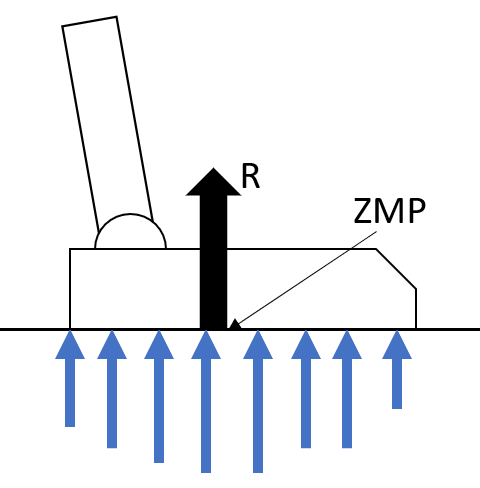
\includegraphics[keepaspectratio, scale=0.6]
  {images/zmp_ilust.png}
  \caption{Illustration of ZMP }
  \label{Fig:zmpillust}
\end{figure}
\newpage

\subsection{テーブル台車モデル}
二足歩行ロボットのモデル化手法として、図\ref{Fig:tablecart}に示すようなテーブル・台車モデルがある。このモデル化により、式\eqref{eq:table-cart}を導ける。ここで、x,x..はロボットの重心位置と重心加速度、hCoMは鉛直方向の重心高さ、gは重心の加速度、pはzmpの位置である。
式\eqref{eq:table-cart}によるモデル化に対し、システムへの入力を重心の躍度(jerk)とすると、二足歩行ロボットは以下のシステムとして表現できる。

\begin{equation}
  p = x - \frac{Z_{c}}{g}\ddot{x}
  \label{eq:table-cart}
\end{equation}


\begin{equation}
  \frac{d}{dt}\begin{pmatrix}
    x \\ \dot{x} \\ \ddot{x}
  \end{pmatrix}
  =
  \begin{pmatrix}
    0 & 1 & 0 \\ 0 & 0 & 1 \\ 0 & 0 & 0
  \end{pmatrix}
  \begin{pmatrix}
    x \\ \dot{x} \\ \ddot{x}
  \end{pmatrix}
  +
  \begin{pmatrix}
    0 \\ 0 \\ 1
  \end{pmatrix}
  u
  \label{eq:teble-cart-system-state}
\end{equation}

\begin{equation}
  p = \begin{pmatrix}
    1 & 0 & -\frac{h_{CoM}}{g}
  \end{pmatrix}
  \begin{pmatrix}
    x \\ \dot{x} \\ \ddot{x}
  \end{pmatrix}
  \label{eq:teble-cart-system-output}
\end{equation}

% \begin{equation}
%   \begin{cases}
%     \dot{x} & = Ax + Bu \\
%     y       & = Cx
%   \end{cases}
%   \label{eq:humanoid-system}
% \end{equation}

\begin{equation}
  \hat{x}_{k}=
  \begin{pmatrix}
    x(kT)\cr \dot{x}(kT)\cr\ddot{x}(kT)
  \end{pmatrix}
  ,
  % {\buildrel\ldots\over{u}}_{k}
  u_{k}
    =
    {\buildrel\ldots\over{x}}(kT)
    , z_{k}=z(kT),
\end{equation}

\begin{equation}
  \hat{x}_{k+1}=
  \begin{pmatrix}
    1&T&T^{2}/2\cr 0&1&T\cr 0&0&1
  \end{pmatrix}
  \hat{x}_{k} +
  \begin{pmatrix}
    T^{3}/6 \\  T^{3}/2 \\ T
  \end{pmatrix}
  u_{k}
\end{equation}

\begin{equation}
  z_{k} =
  \begin{pmatrix}
   1 & 0 & \frac{h_{CoM}}{g}
  \end{pmatrix}
  \hat{x}_{k}
\end{equation}

\begin{figure}[hbtp]
  \centering
  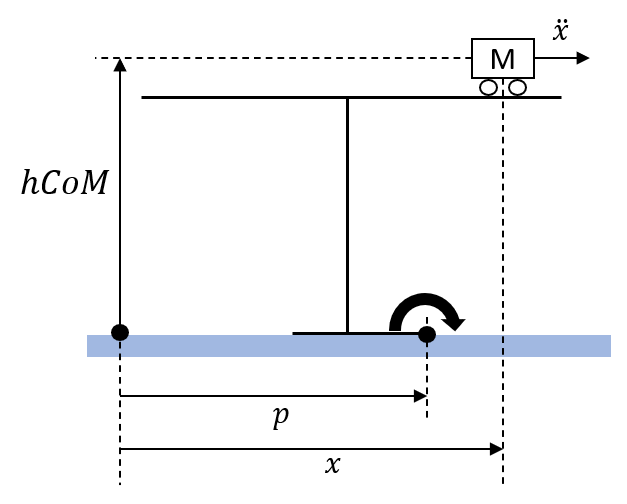
\includegraphics[keepaspectratio, scale=0.6]
  {images/table_cart_hcom.png}
  \caption{Illustration of table-cart model }
  \label{Fig:tablecart}
\end{figure}



\newpage

\subsection{予見制御による歩行パターン生成手法}
上記のZMPとテーブル台車モデルの概念を利用した歩行パターン生成手法として、kajitaらによる予見制御を利用した歩行パターン生成手法\cite{PREVIEW}がある。kajitaらによる手法では式()によって表現したロボットのダイナミクスに対して、予見制御理論によって以下の評価関数式()、を最小化する制御入力(二足歩行ロボットの歩行パターン)を得る。

(式を入れる)
\begin{equation}
  \min_{{\buildrel\ldots\over{x}}_{k},{\buildrel\ldots\over{x}}_{k+1},\ldots}\sum_{i=k}^{\infty}{1\over 2}Q\left(z_{i+1}-z_{i+1}^{ref}\right)^{2}+{1\over 2}R{\buildrel\ldots\over{x}}_{i}^{2}
  \label{eq:mpc_valuefunc}
\end{equation}

式\eqref{eq:mpc_valuefunc}内、$z$はZMPの位置、$z^{ref}$はZMPの目標位置、$u$は入力である重心の躍度(jerk)を示す。

\subsection{MPCを利用した歩行パターン生成手法}
本研究では、kajitaらによる予見制御を利用した歩行パターン生成手法\cite{PREVIEW}をMPCによって拡張した、Wieberらによる手法\cite{WIEBER}を実装する。ここでは、その手法\cite{WIEBER}について説明する。

まず、MPCは最適制御の一種であり、無限長の区間に渡る最適化問題を解く代わりに、有限長の区間で最適化問題を解いて最適入力を得る手法である。有限区間の最適化問題であるがゆえに、陽に表現した制約を考慮しながら最適化問題を解く事ができるのが特徴である。また、有限区間での最適化問題を解く際には、有限区間に渡る未来の状態、ないしは出力の予測値を利用して最適化を行う。
以下の式()で表されるダイナミクスからなるシステムでは、予測は以下の式で表される。

Wieberらによる手法\cite{WIEBER}では、式()のダイナミクスを元に、以下を評価関数とする。

(式を入れる)
ここで、pref は目標zmp(目標出力)、pは現在のzmp(現在の出力)x…は重心のjerk(入力)となる。
この式()で表される評価関数とkajitaらによる手法の式()の評価関数の違いは評価区間である。
kajitaらの式()では評価区間が無限区間であるのに対して、MPCを利用したwieberらの式()は評価区間の長さがNとなっている。

上記の評価関数に対して、以下の式で表される不等式制約を与える。
(式を入れる)
(式を入れる)

上記の不等式制約では、入力と出力に対して、上下限が設定される。入力の上下限はモーターの最大速度等、ロボットの特性によって決定される。ここで、出力制約はZMPの支持多角形内での位置に対しての制約となる。ZMPが支持多角形の境界部にある時に、ロボットは転倒を始めるので、支持多角形の境界部から一定の距離を取った範囲が制約の範囲となる。

上記の式()の評価関数を二次計画法の問題として捉え、式()と式()からなる制約を考慮して制御ステップ毎に解く事でそのステップでの最適入力を得る。